\documentclass[conference]{IEEEtran}
\IEEEoverridecommandlockouts
 
\usepackage{cite}
\usepackage{amsmath,amssymb,amsfonts}
\usepackage{algorithmic}
\usepackage{graphicx}
\usepackage{textcomp}
\usepackage{xcolor}
 
\usepackage{url}
\usepackage{hyperref}     
\usepackage{footnote}       
\usepackage{graphicx}

\usepackage{array}
\usepackage{booktabs}
\usepackage{multirow}
\usepackage{caption}
\usepackage{tabularx}

\usepackage[left=25mm,right25mm,top=25mm,bottom=25mm,work=a4work]{adjustbox}


 


\def\citepunct{], [}
\def\citedash{]--[}



\def\BibTeX{{\mathrm B\kern-.05em{\sc i\kern-.025em b}\kern-.08em T\kern-.1667em\lower.7ex\hbox{E}\kern-.125emX}} 

%\setlength{\parindent}{0pt}
%\setlength{\parskip}{0.5\baselineskip}
\begin{document}


\title{HeartPal: An Embedded System for Real-Time Atrial Fibrillation Diagnosis Using a Multimodal Approach to ECG Data}

\author{\IEEEauthorblockN{Monalisa Akter}
\IEEEauthorblockA{\textit{Electrical and Computer Engineering} \\
\textit{North South University}\\
Dhaka, Bangladesh \\
monalisa.akter@northsouth.edu}
\and
\IEEEauthorblockN{Nayeema Islam}
\IEEEauthorblockA{\textit{Electrical and Computer Engineering} \\
\textit{North South University}\\
Dhaka, Bangladesh\\
nayeema.islam@northsouth.edu}
\and
\IEEEauthorblockN{Abdul Ahad}
\IEEEauthorblockA{\textit{Electrical and Computer Engineering} \\
\textit{North South University}\\
Dhaka, Bangladesh \\
Ahad.abdul01@northsouth.edu}
\and
\IEEEauthorblockN{Md. Asaduzzaman Chowdhury}
\IEEEauthorblockA{\textit{Electrical and Computer Engineering} \\
\textit{North South University}\\
Dhaka, Bangladesh \\
asaduzzaman.Chowdhury@northsouth.edu}
\and
\IEEEauthorblockN{Fahim Foysal Apurba}
\IEEEauthorblockA{\textit{Electrical and Computer Engineering} \\
\textit{North South University}\\
Dhaka, Bangladesh\\
fahim.apurba@northsouth.edu}
\and
\IEEEauthorblockN{Riasat Khan}
\IEEEauthorblockA{\textit{Electrical and Computer Engineering}\\
\textit{North South University}\\
Dhaka, Bangladesh \\
riasat.khan@northsouth.edu}
}


\maketitle

\begin{abstract}

In the face of global health problems, cardiovascular disease is a severe risk to human health. To address this problem, we proposed a novel method for diagnosing Atrial Fibrillation, which is the pre-stage of major heart diseases. Our system comprises an embedded system comprising an ESP8266 microcontroller and an AD8232 single-lead ECG sensor to take real-time ECG samples. In addition, we have used a deep learning model that can differentiate Atrial Fibrillation from Normal ECG signals. The proposed method includes ECG signal recording in real-time and a Multimodal model trained on the PTB- XL dataset, which uses a step approach of CNN-bidirectional- LSTM for numeric ECG series and VGG16 for image-based ECG representations. A fusion layer has been incorporated into the Multimodal model for better detection of Atrial Fibrillation, which produces state-of-the-art outcomes with 94.07\% accuracy and 0.94 F1-score. This study demonstrates the effectiveness of a multimodal approach in increasing the accuracy of diagnosis of cardiovascular diseases in real-time. Furthermore, for edge devices, we have distilled the knowledge to train a small student model named CNN-LSTM by keeping a large CNN-BiLSTM model as a teacher, which successfully performs with 83.21\% accuracy. Our work represents a substantial leap towards competent and preventive advanced cardiovascular health management. 

\end{abstract}

\begin{IEEEkeywords}
Atrial Fibrillation (AFib),
Cardiovascular Disease,
ECG Signal Processing,
CNN-bidirectional-LSTM,
Multimodal Approach,
Remote Health Monitoring.
\end{IEEEkeywords}

\section{Introduction}
Cardiovascular disorders remain the leading cause of death globally, accounting for approximately 17\% of all deaths \cite{drozd2021causes}. The World Health Organization estimates there are 9 million deaths ascribed to these conditions each year. Atrial fibrillation (AF) is a common arrhythmia that significantly increases the risk of stroke and heart failure \cite{chung2020atrial}. Hence, proper management of AF entails early identification of the condition and constant supervision to prevent serious consequences. However, existing ECG monitoring systems are expensive, complicated, and require hospital visits, making them inadequate for continuous real-time monitoring, especially in non-clinical settings.

IoT technology has rapidly accelerated a drastic change in the healthcare sector by establishing portable health monitoring systems \cite{dalloul2023review}. These IoT-based systems enable constant surveillance of the patient's condition, timely notification, and significantly better outcomes \cite{boikanyo2023remote}. Despite their potential, current IoT-based ECG monitoring solutions often fail to provide a full range of Multimodal diagnostic tools designed for Atrial fibrillation (AF) identification. 

Recent research indicates that there have been significant advancements in the healthcare sector in deep learning and IoT technology. For example, they developed a low-cost portable ECG monitoring system with deep learning algorithms to detect arrhythmia with an overall accuracy of 97.57\% \cite{mehra2007global}. Furthermore, they employed affordable components such as Raspberry Pi, ESP8266, and ECG sensors in this system to demonstrate the feasibility of creating cost-effective and portable remote monitoring systems \cite{ahsanuzzaman2020low}.

In this work, we introduced HeartPal, an embedded system for real-time atrial diagnosis based on a multimodal analysis of ECG data. The system combines the latest machine learning techniques, IoT devices, and interfaces to provide a complete solution to continuous heart monitoring. We designed HeartPal to overcome the drawbacks of conventional ECG systems and become a very effective, portable, and accurate tool for the early diagnosis and control of Atrial fibrillation (AF), which will help to enhance the quality of life of patients and decrease the costs of health care services.

This work describes a novel approach to detecting stroke and coronary heart disease based on ECG-based biosignals. This system uses embedded technologies and machine learning to analyze ECG data in real-time, which is recorded through an integrated method. The interpretive process is done through the integration of hardware and machine learning, which is easy to use and hence makes it possible for people to keep track of their heart health at a low cost. The findings of the semantic analysis can be incorporated into this system to offer an objective diagnosis and potentially prognostic therapy to medical professionals. The key contributions of our work include:

\begin{itemize}
    \item \textbf{Multimodal ECG Data Analysis:} The enhancement of HeartPal increases the AF detection rate and credibility with the help of the numerical and image data forms of ECG signals in contrast to the single-modality systems.
    \item \textbf{Real-time Monitoring and Alerts:} The exploration and application of real-time ECG signal analysis immediately alerts patients and healthcare providers of potential AF episodes and timely treatment.
    \item \textbf{Portable and Cost-effective Solution:} The system is portable and effective, making it suitable for home use and in areas with limited access to health care, thus filling the existing void in healthcare.
    \item \textbf{Advanced Deep Learning Algorithms:} The system employs signal processing and classification algorithms like CNN-LSTM and VGG-16 for efficient and sensitive identification of Atrial fibrillation (AF).

\end{itemize}

The subsequent sections of this work state a comprehensive methodology, an experimental setup, and elaborated results demonstrating the effectiveness of HeartPal in the advanced healthcare domain. Thus, by eliminating the shortcomings of the existing systems and introducing new options, HeartPal will be advantageous in the early detection and treatment of atrial fibrillation, which will produce a positive impact on the prognosis and quality of life of the patient.

The remainder of this work is structured as follows. Section II further discusses the real-time stroke prediction and heart disease diagnosis using ECG data and machine learning presented in this research. Finally, Section V concludes the work, offering information on potential future research directions.


\section{Related Work}
This section narrates a brief description of recent developments in real-time stroke prediction and heart disease diagnosis, with a special emphasis on methodologies that use time series ECG data and machine learning for stroke prediction.

Yu et al. \cite{yu2022ai} developed a system that used real-time ECG and PPG multimodal biosignals to detect stroke and evaluate the health status of the individuals. Their strategy included a signal sensor for assessment and reporting, using a sample of 287 stroke patients and 287 elderly patients without stroke. First, they extracted features based on the peak values obtained from the ECG and PPG signals. The authors then incorporated a method to capture, record, and wirelessly transfer multimodal real-time biosignals to a server. Lastly, they used a machine learning algorithm to predict prognostic symptoms of stroke in aged people in real-time, and the validation was 91.56\% for the C4.5 decision tree, 97. 51\% for Random Forest and 99. 15\% for CNN-LSTM models using 10-fold cross-validation data sets.

Choi et al. \cite{choi2021deep} presented a deep-learning approach to predict stroke from raw real-time biosignals without frequency characteristics. They gathered raw EEG data from a hospital emergency medical center for people 65 years and older, preprocessed at a sampling rate of 1000 Hz from six channels, and derived power and relative values from the frequency attribute. They employed four types of deep learning models, and the best model was the CNN-bidirectional LSTM model. They also found a way of sending data to a server, where the model analyzed it to make the predictions. Eventually, their CNN bidirectional LSTM model achieved an accuracy of 94\%, which was a 6.0\% low false positive rate (FPR) and a 5. 75\% false negative rate (FNR). At the same time, it decreases the cost of stroke testing in everyday life.

Lavanya et al. \cite{lavanya2023wearable} proposed a wearable sensor-based edge computing framework to identify cardiac arrhythmia and the prognosis of acute stroke in IHS. Furthermore, focusing on the preprocessing and deep learning-based assessment at the edge computing layer, they enhanced the classification accuracy for acute stroke prediction. They laverized The cloud servers' application for storing and sharing healthcare data between hospitals, institutions, families, and professionals was discussed. Their approach included wireless ECG monitoring through wearable devices and sensors with the help of microcontrollers and wavelets for signal extraction and signal-to-noise ratio (SNR) improvement. ANN, decision trees, Naive Bayes, KNN, and Support Vector Machine algorithms were employed to identify the risk of cardiovascular disease, and the proposed edge computing-based technique obtained 99.3\% precision, 99.1\% specificity, and 99.4\% sensitivity in 250 patient records.

Shin et al. \cite{shin2022lightweight} proposed an ensemble algorithm for arrhythmia diagnosis with the MobileNet architecture to smooth the work in mobile applications. They successfully enhance the ECG signal measurements taken over a short period by employing the matching pursuit algorithm. Using the MIT-BIH database, their proposed ensemble classifier with MobileNetV2 and BILSTM performed 91.7\% perfection and approximately 0.92 F1-score. Eventually, the attempt was to make it easier for people with a tight schedule to manage their health.

Choi et al. \cite{choi2021machine} presented a machine-learning approach to monitor the health of older people during their daily activities using vital EEG signals for stroke and other diseases. Their system had a user or caregiver layer for visualization and a layer for inputting wave frequency. They obtained raw EEG data and preprocessed it using FFT, which obtained power values from raw spectra; they used a Random Forest algorithm with quartiles and Z-score normalization and got an accuracy of 92.5\% stroke prediction accuracy.

Zhou et al. \cite{zhou2024multimodal} transformed ECG signals into modal images using GAF, RP, and MTF methods and then inputted them into a TA CNN-based model with FCA for better preservation detail in multimodal ECG applications. Eventually, this method achieved 99. 6\% of accuracy in working with the MIT-BIH arrhythmia database, which consisted of five different arrhythmia classes. Then, they demonstrated the possibility of using multimodal fusion in ECG analysis.

Zhang et al. \cite{zhang2023multimodal} proposed a deep neural network using ECG and PCG signals for event classification. Combining the features from both signal types, their model, trained on the PhysioNet database, obtained 92.3\% accuracy, sensitivity of 97\%, specificity of 99\%, precision of 98\%, and F1 score of 98\%.

Ahmad et al. \cite{ahmad2021ecg} used two multimodal fusion approaches, namely Multimodal Image Fusion (MIF) and Multimodal Feature Fusion (MFF), to classify ECG heartbeat. Furthermore, they transformed  ECG signals into images using GAF, MTF, and RP techniques; MIF fused these images for CNN input; and MFF extracted features for classification using SVM. Their approach achieved 99.7\% accuracy in working with the MIT-BIH and PTB datasets.

Han et al. \cite{han2023multimodal} presented a multimodal multi-instance learning neural network (MAMIL) to classify long-term ECG signals using original ECG signals and their GAF images as inputs. The MIL approach ensured no information loss, considering each heartbeat on the ECG and the GAF patch as instances. CNN extracted features and an attention-based fusion method combined them for the final classification, which was superior to other deep learning-based models in long-term ECG datasets.

Mert and Akan \cite{mert2023time} proposed a new vision transformer model to identify fibrillation from lead ECG signals. They employed wavelet-based synchrosqueezing transform (WSST) for the time-frequency domain analysis and generated time-frequency images from ECG signals. They evaluated these signals using a developed vision transformer (ViT) model. This system achieved a precision of 95.8\% in identifying fibrillation and high sensitivity, specificity, recall, and F1 scores.

Żyliński et al. \cite{zylinski2023design} proposed an edge computing algorithm for atrial fibrillation detection on microcontrollers, like the ARM Cortex-M4, which enables efficient implementation of machine learning classifiers for atrial fibrillation detection, with notable advantages in power efficiency, data privacy, and system costs. However, difficulties like false-positive detection and the clinical significance of detected arrhythmias remain.

Obeidat et al. \cite{obeidat2023embedded} proposed a cost-effective, portable ECG diagnostic system utilizing Raspberry Pi, offering wireless and wired interfaces for real-time heart monitoring to lead the development of recent advancements. So, this embedded system integrates analog and digital components for signal conditioning and conversion, providing accurate ECG measurements on a graphical display. The system's ability to detect heart abnormalities efficiently highlights its potential in various medical settings. Eventually, this system performed with vast effectiveness.

Su et al. \cite{su2023ecg} introduced an ECG acquisition and analysis system that combined traditional machine learning models, including logistic regression, SVMs, and XGBoost, with deep learning models like CNNs and LSTMs for enhanced ECG signal classification for the recent advancement. By applying the fusion of these models, achieving a classification accuracy of 99.13\% was the core contribution of the work. Eventually, this study highlights the potential of integrating machine learning with feature engineering to improve ECG signal analysis and emphasizes future work on portability and model optimization.

The literature reviews have emphasized the extensive research on different heart issues using deep learning techniques. However, notable gaps were detected when working with ECG data. Furthermore, most articles didn't work with taking real-time ECG signals and predicting atrial fibrillation simultaneously. Moreover, they didn't explore algorithms or approaches for the diverse forms of the same dataset, such as the multimodal approach. In addition, they didn't work for the edge devices and work with real-time ECG input taking. Furthermore, none of the articles work with this kind of numeric series values ECG dataset, which is very difficult to classify.

\section{Proposed Methodology}

\subsection{Hardware Components}

Our proposed system has a hardware part. This part has the role of taking the real-time ECG signal as input. However, this is not a ready hardware system. Eventually, we had to collect different parts from the market and set them up as a complete system as we wished. In Table \ref{table:Hardware-1}, we have displayed the name, the quantity, and the price of the components. Finally, we have displayed the total cost for the hardware system.

\begin{table}[!ht]
\centering
\caption{Approximate cost of the hardware device.}
\begin{tabularx}{\columnwidth}{|X|X|X|X|}
\hline
\textbf{Component} & \textbf{Unit Price (in USD)} & \textbf{Quantity} &  \textbf{Total Cost} \\
\hline
ESP8266 Microcontroller & 4.50 USD & 1 & 4.50 USD\\
\hline
AD8232 ECG Sensor with Electrodes & 8.00 USD & 1 & 8.00 USD\\
\hline
Raspberry Pi Model 4B (Complete Set) & 130.00 USD & 1 & 130.00 USD \\
\hline
9V Battery & 1.00 USD & 1 & 1.00 USD\\
\hline
Buck Converter & 1.30 USD & 1 & 1.30 USD\\
\hline
Biomedical Sensor Pads & 0.09 USD & 3 & 0.27 USD \\
\hline
Jumper Wires & 0.03 USD & 10 & 0.30 USD\\
\hline
 & & Subtotal Cost & 144.07 USD\\
\hline
\end{tabularx}
\label{table:Hardware-1}
\end{table}
 
The proposed system includes several critical hardware components for effective and precise ECG monitoring. The core of this configuration is the AD8232 single-lead ECG sensor that employs three biomedical electrode pads to capture the heart's electrical signals. Using the AD8232 sensor, we recorded the real-time ECG signals. Then, we fed the signals to the ESP8266 Wi-Fi microcontroller. Eventually, this microcontroller acted as a relay and transmitted the gathered data to the Raspberry Pi 4 B for further signal processing.
On the other hand, the ESP8266 was directly connected to the Raspberry Pi 4 B via a USB cable to facilitate data transfer. Then, we loaded the Arduino Integrated Development Environment (IDE) into the Raspberry Pi operating system to read the serial data on the Raspberry Pi. This setup allowed real-time data acquisition and processing on the Raspberry Pi platform.
In addition, we incorporated a 9V battery into the circuit to supply power to the entire system. Then, we controlled the voltage and minimized it to 5V using a buck converter to supply all the required power to the components. Eventually, this configuration provided operational stability and portability of the system, which can be used for continuous ECG monitoring in different environments. In Fig. \ref{fig-1:Hardware architecture}, we have shown the design of the whole hardware system with the labeled components.

\begin{figure}[htbp]
\centerline{\includegraphics[width=3.5in]{1-Hardware Architecture.png}}
\caption{Proposed Architecture of the hardware system.}
\label{fig-1:Hardware architecture}
\end{figure}


\subsection{Real-time ECG Monitoring and Data collection}

In the implementation phase, the system uses three electrodes as main inputs; these electrodes are positioned on the necessary body parts to obtain the most accurate data. We connected these electrodes to the AD8232 ECG sensor that recorded the cardiac signals and relayed them to the ESP8266 microcontroller. The ESP8266 module then receives the data and displays the ECG readings obtained on the serial monitor of the Arduino Integrated Development Environment.

In Figure 11, the $y$-axis is the amplitude of the ECG signal in the raw ADC values from 0 to 1023 for a 10-bit ADC. These values represent the electrical activity of the heart at each sampling point. The x-axis represents the sample numbers, which were calibrated in terms of time by dividing with the sampling rate. Every point on the x-axis represents one sample taken by the ADC for the given signal.

\begin{equation}
\ T = \frac{n}{fs} \
\end{equation}

Here, \( T \) represents the duration, \( n \) is the number of samples taken, and $f_s$ is the sampling rate, which in our case is 99 Hz.

Next, to improve the raw ECG signal, we converted the ADC values to voltages using the reference voltage of 3.3V that the AD8232 sensor uses.

\begin{equation}
\text{Voltage}, V = \left(\frac{\text{ADC\_value}}{1023}\right) \times 3.3 
\end{equation}

The proposed system includes several critical hardware components for effective and precise ECG monitoring. The core of this configuration is the AD8232 single-lead ECG sensor that employs three biomedical electrodes. After that, we subtracted the mean voltage from the converted signal to remove the baseline wander. We used a bandpass filter with a low cutoff frequency of 0.5 Hz and a high cutoff frequency of 40 Hz to further filter the signal. This filtration was very useful in eliminating high-frequency noise and low-frequency drift, hence improving the quality of the ECG signal. Finally, we generated a time vector to map each sample to its corresponding time point using the following formula:

\begin{equation}
t = \left[ \frac{0}{fs}, \frac{1}{fs}, \frac{2}{fs}, \frac{3}{fs}, \ldots, \frac{(n-1)}{fs} \right] 
\end{equation}

Here, \( n \) is the number of samples taken, and $f_s$ denotes the sampling frequency.

During the development process, we used several iterative methods to fine-tune signal processing and obtain the best response of the ECG signal. This iterative process made the system more reliable in capturing and processing the ECG data since we repeated it several times.

\subsection{Experimental Setup}
This embedded system has been tested and implemented in real world conditions.

\begin{figure}[htbp]
\centerline{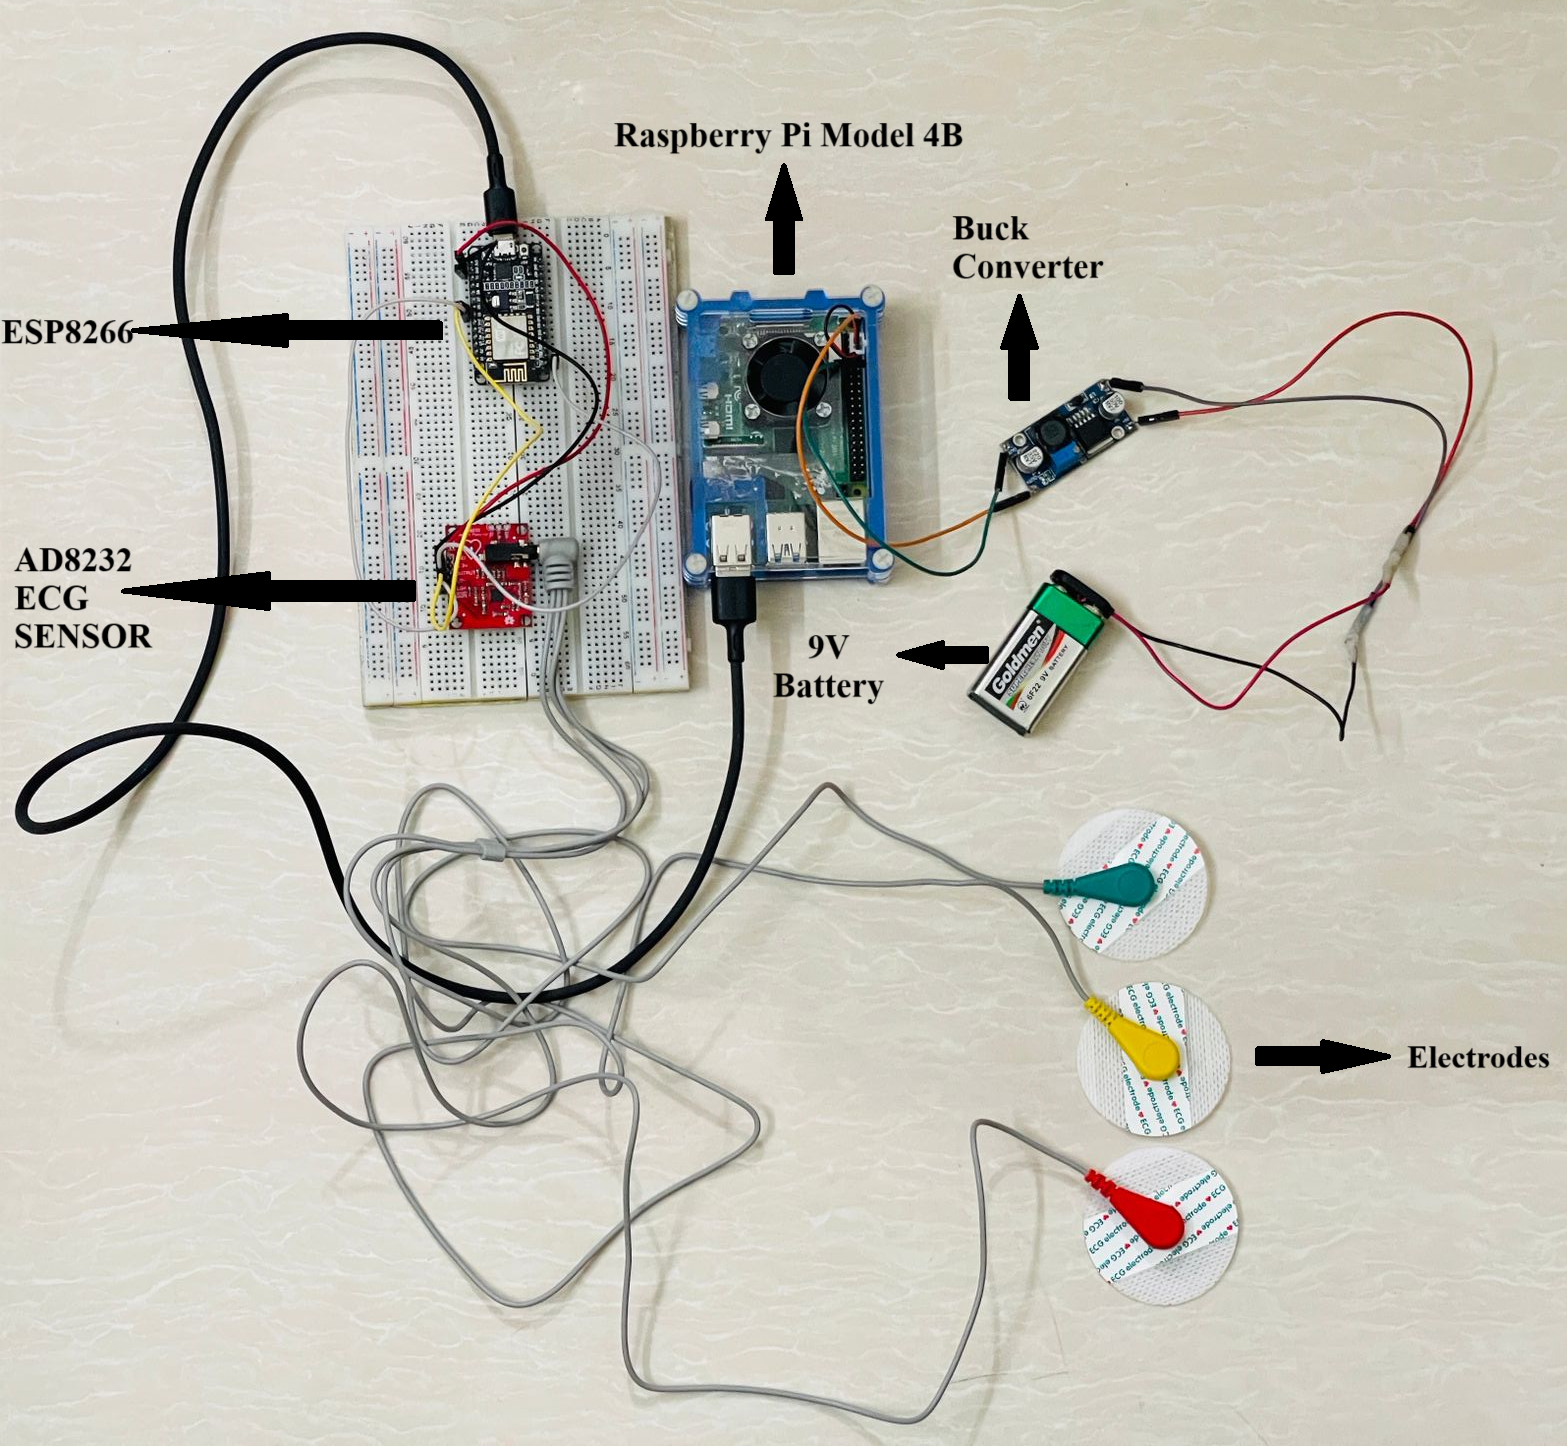
\includegraphics[width=3.5in]{2-Hardware Setup.png}}
\caption{Hardware setup.}
\label{fig-2:Hardware Setup.}
\end{figure}

Fig. \ref{fig-2:Hardware Setup.} shows a complete hardware setup for taking real-time ECG data for only three leads. These three leads will generate only three ECG signals. We take three of the twelve leads because we don't need all twelve to detect atrial fibrillation.

There are two standard techniques for placing electrodes for ECG recordings. The study of Fig. \ref{fig-3: Electrodes' Placement.} shows the procedure for placing the electrodes on a patient's body. So, the electrodes should be placed based on the procedure outlined in this work.

\begin{figure}[htbp]
\centerline{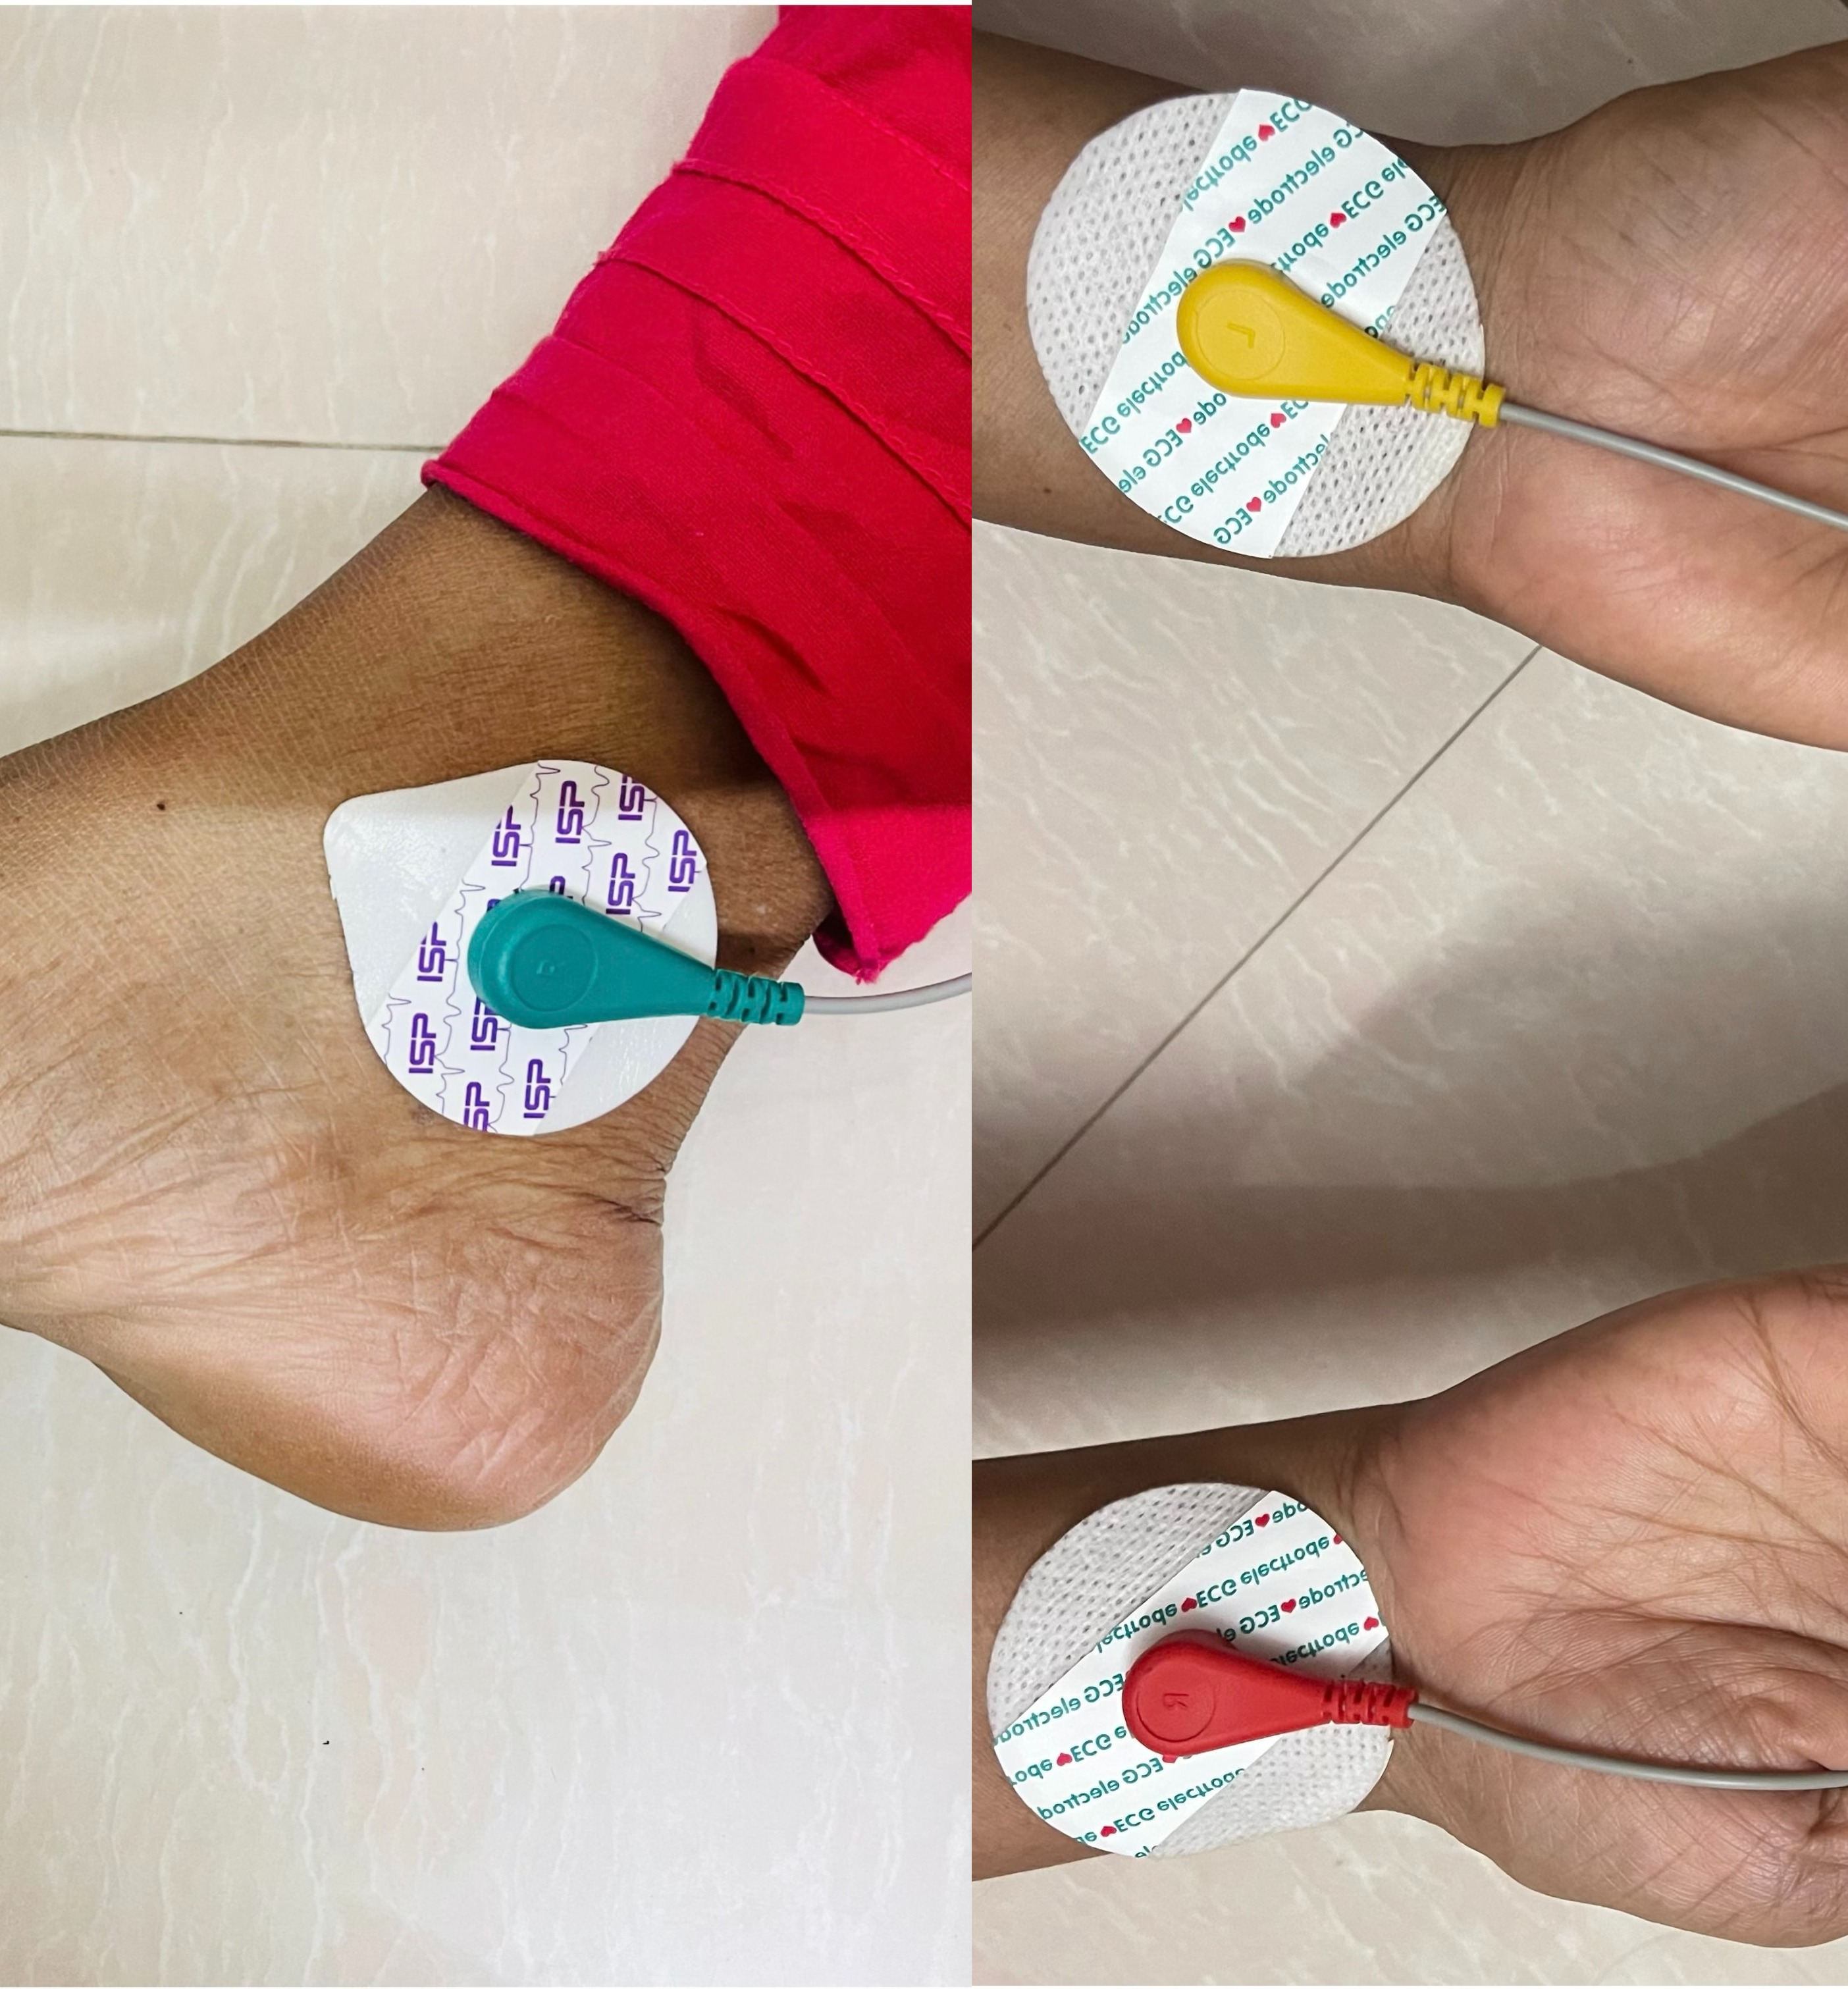
\includegraphics[width=3.5in]{3-Electrods' Placement.jpg}}
\caption{Placement of the electrodes.}
\label{fig-3: Electrodes' Placement.}
\end{figure}

The patient should be relaxed and still during the ECG recording to avoid interference with the results obtained. Eventually, this relaxation will reduce the chances of interference from movement artifacts and other noises that may distort the ECG signal. Hence, the quality of the obtained results will improve.

\subsection{Dataset}

The study uses the PTB-XL ECG signal database \cite{wagner2020ptb}, which contains atrial fibrillation detection data and is available on the PhysioNet website. This database includes signal values from 12 leads: The lead names include I, II, III, aVF, aVR, aVL, V1, V2, V3, V4, V5, and V6, which consists of 21,799 clinical ECG records and a metadata file. Furthermore, we collected the recorded signals from 18,869 patients with records available at two sampling frequencies of 100 Hz and 500 Hz, which were 10s in duration. Specifically, we used 100-Hz signals in our study.

\begin{figure}[htbp]
\centerline{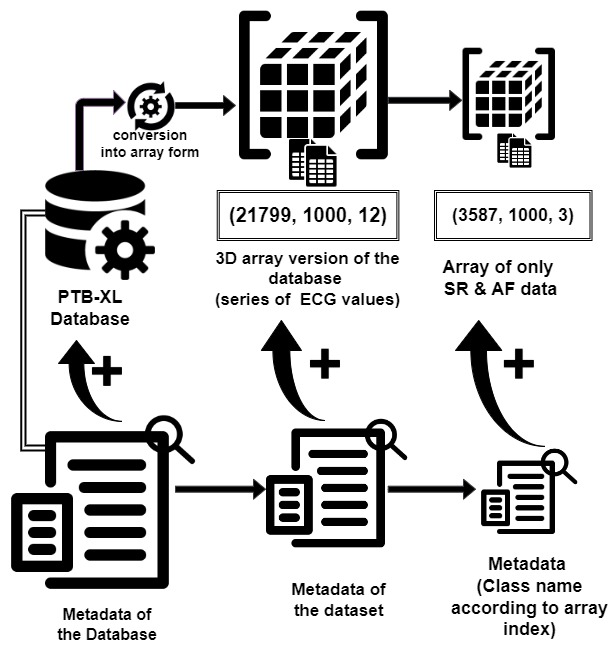
\includegraphics[width=3.5in]{4-Conversion.jpg}}
\caption{Conversion of PTB-XL database to dataset.}
\label{fig-4:Conversion}
\end{figure}

In Fig. \ref{fig-4:Conversion}, we show the conversion of the dataset from the database. To make the database usable, we have formed a 3D array of series values of ECG data along with a metadata file, which contains the type of diagnosis for each sample. This array has a shape of (21,799, 1000, 12), where 21,799 is the number of samples, 1000 is the data points per signal (100 Hz $\times$ 10 s), and 12 is the number of leads. The normal ECGs were 9514, myocardial infarctions 5469, STTC 5235, conduction disturbances 4898, and hypertrophy 2649 samples. However, in our study, we were interested in differentiating between normal sinus- rhythm and atrial fibrillation. Thus, we obtained 2,000 normal-sinus-rhythm samples and 1,587 atrial fibrillation samples, which gave a final dataset of 3,587 samples with a size of (3,587, 1000, 12).

\begin{figure}[htbp]
\centerline{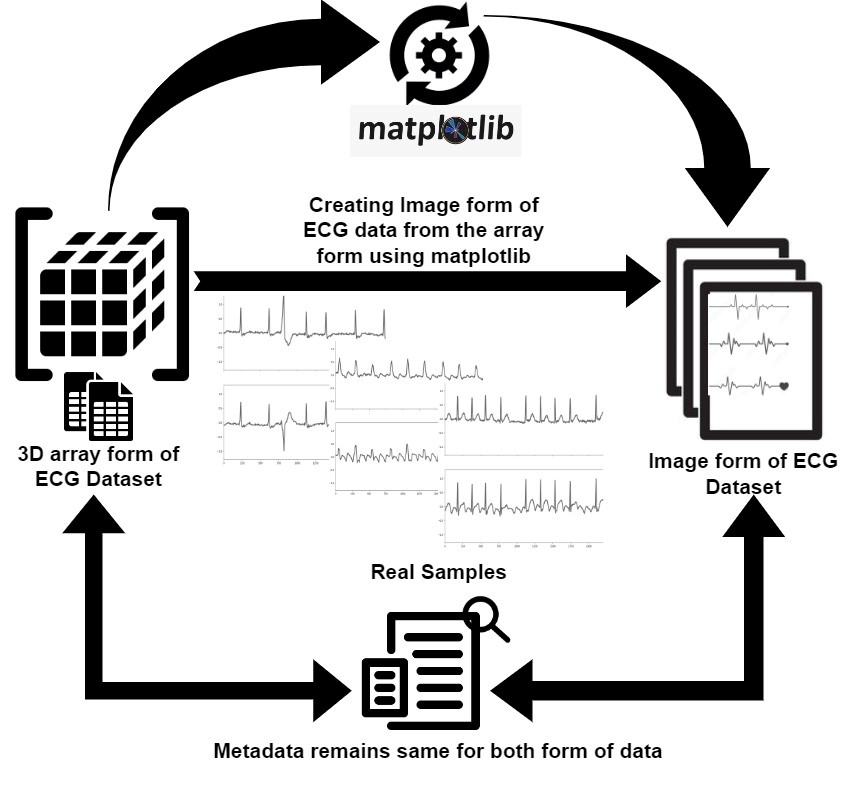
\includegraphics[width=3.5in]{5-Generating Image Data.jpg}}
\caption{Generating image data from 3D array data.}
\label{fig-5:Generating Image}
\end{figure}

The literature \cite{ramkumar2018atrial} said that leads V1 and II are essential to identify Atrial Fibrillation. ). However, only 3 of the leads V1, V5, and II are enough to detect atrial fibrillation \cite{kristensen2016use}. Therefore, we added lead V5 and limited the dataset to the required leads to eliminate noise. This process resulted in the final filtered dataset with the shape (3,587, 1000, 3). We also cleaned the metadata file to contain only the diagnosis type, where 0 is normal sinus rhythm, and 1 is atrial fibrillation.

Fig. \ref{fig-5:Generating Image} shows the process of generating ECG images from the raw ECG signals or 3D array data. For visualization, we created image forms of the ECG data from the array data using Matplotlib and got 3587 ECG graph images for 3587 array instances. This dual-format data approach enables a new multimodal analysis method that improves the capacity of our model to identify atrial fibrillation correctly.

\subsection{Exploratory Data Analysis (EDA)}

Since there were two diagnostic classes, the task was binary classification. The number of instances of both classes was approximately similar. Specifically, this dataset contains 2,000 normal sinus rhythm and 1,587 atrial fibrillation samples. Since the ratio of these classes is not less than half, we could consider the data distribution for the classes was satisfactorily balanced for the analysis.

\subsection{Preprocessing Data}

Before feeding data to the model, data preprocessing is an essential process at the data preparation stage. Therefore, we need some preprocessing stuff to prepare data for model training. Eventually, we properly preprocessed both forms of our data to enhance the performance of the laborized models.

\begin{figure}[htbp]
\centerline{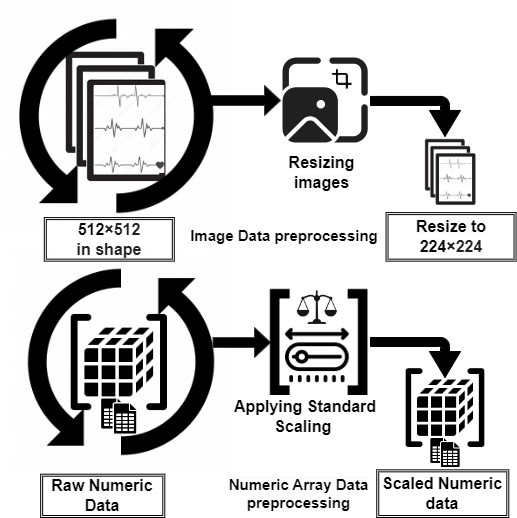
\includegraphics[width=3.5in]{6-Preprocessing Data.jpg}}
\caption{Preprocessing both forms of data.}
\label{fig-6:Preprocess Data}
\end{figure}

As illustrated in Fig. \ref{fig-6:Preprocess Data}, we have preprocessed and prepared for training models. In detail, we reshape the image data into 224$\times$224 size from  512$\times$512 size so that it could fit in models easily. Moreover, 224$\times$224 is a standard size for less time consumption and cost-effectiveness. A size of 224$\times$224 is useful when the topic comes to reducing the cost of training time and computational load while still maintaining data quality. On the other hand, we have scaled the 3D array form of numeric series data using a commonly used standard scaling method for better model fitness. This standard scaling method standardizes the data to have a mean of zero and a standard deviation of one, which is very important to improve the performance and convergence of machine learning models. This method did it by normalizing the data so that all features had the same impact on the model training process, thus improving the model's ability to learn and generalize from the data.

\subsection{Train-Test Split}


\begin{figure}[htbp]
\centerline{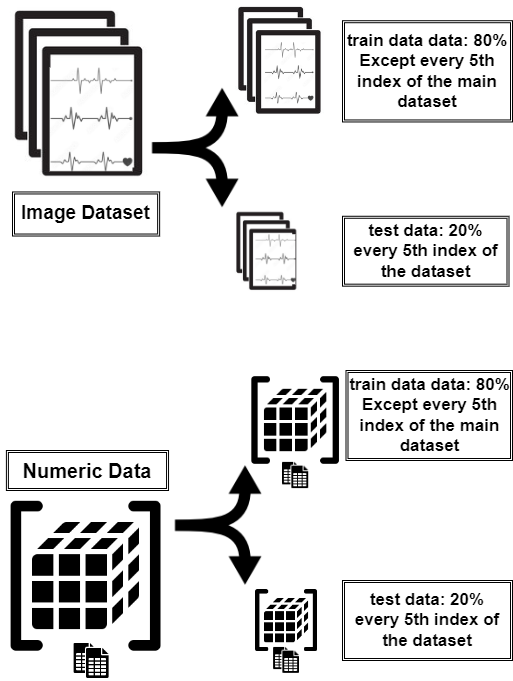
\includegraphics[width=3.5in]{7-Splitting Dataset.png }}
\caption{Splitting both forms of data into train and test.}
\label{fig-7:Splitting Dataset}
\end{figure}


Fig. \ref{fig-7:Splitting Dataset} illustrates that we utilized an unorthodox technique to split both forms of the datasets into train and test. Therefore, we placed every 5th index of the original dataset into the test dataset and the rest of the indexes in the train set. For instance, one-fifth equals 0.2. Accordingly, we allocated approximately 20\% of the data to the test and 80\% of the data to the train set. We applied this technique to both cases to ensure that the indexes were aligned and the training and testing subsets were in harmony. Eventually, it allows us to pursue a multimodal approach. In this way, we guarantee the alignment in the index allocation, which allows for a coherent multimodal approach in our analysis.

\subsection{Train ML Models}

The study wanted to determine deep learning models with validated data-type images and numerical data on a training dataset. Image data analysis was focused on the comparison between convolutional neural networks (CNNs) and Visual Transformers, highlighting the trade-off performance of ResNet32 and Vision Transformer (ViT) for image classifiers with VGG16 showing an edge in terms of higher accuracy. However, it also has greater computational efficiency. The human label was necessary on numerical data arrays for tasks of Long Short-Term Memory (LSTM), CNN-LSTM, and also the concurrent usage between LSTM with conventional convolutional architectures in either mono-directional or bi-directional temporal observation, namely CNN-Bi-LSTMs to evaluate numbers. Acquired results indicated maximum success using both sharable procedures, targeting a couple of successful experiences by BiLSTMs nature. These demonstrate that CNNs and transformers can both be used for image data analysis, as well as those of sequential numeric data processing combined of a CNN with an LSTM model. In-depth analysis led to identifying the most appropriate models for a specific data set, resulting in reliable and effective classification solutions for the datasets.


\subsection{VGG16 model (Visual Geometry Group 16)}

VGG16 is a CNN created by the Visual Geometry Group, and it is mainly used for image classification. It contains 16 weight layers, of which 13 are convolutional, and three are fully connected layers.



\begin{figure}[htbp]
\centerline{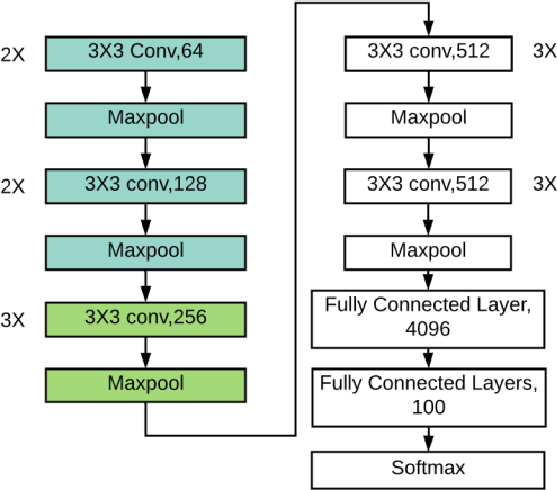
\includegraphics[width=3.5in]{8-VGG16.png}}
\caption{VGG16 model architecture.}
\label{fig-8:VGG16}
\end{figure}

The architecture of VGG16, as shown in Fig. \ref{fig-8:VGG16}, consists of 13 convolutional layers where each layer has 3$\times$3 kernel size with a stride of 1 and padding of 1 to maintain the spatial dimension. All the convolutional layers are followed by a Rectified Linear Unit (ReLU) to introduce linearity. On the other hand, the model contains the activation functions in its structure to introduce nonlinearity.

Moreover, the model has five max-pooling layers, which down-sample the feature maps by applying a 2$\times$2 window with a stride of 2. Furthermore, the first two of the fully connected layers had 4096 neurons, and the last layer had 1000 neurons. These layers help to learn higher-level features in the data hierarchy.

The output layer uses the softmax activation function to obtain class probabilities. Thus, VGG16 is suitable for tasks that involve accurate classification across various image datasets.

\subsection{CNN-BiLSTM Model}

CNN-BiLSTM is a model that combines CNNs and BiLSTMs to learn features from sequential data and temporal dependencies. It is most effective for tasks that require the identification of patterns and sequences within the data.



\begin{figure}[htbp]
\centerline{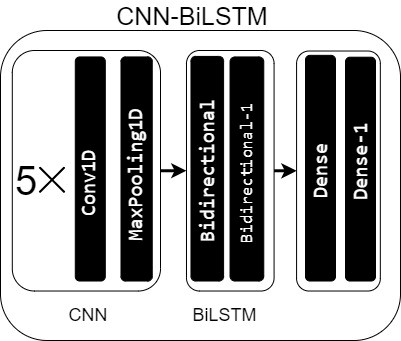
\includegraphics[width=3.5in]{9-CNN-BiLSTM.jpg}}
\caption{Architecture of the CNN-BiLSTM model.}
\label{fig-9:CNN-BiLSTM}
\end{figure}

As shown in Fig. \ref{fig-9:CNN-BiLSTM}, the CNN-BiLSTM framework consists of the following black-colored layers in Fig. \ref{fig-9:CNN-BiLSTM}. The first layer is Conv1D-64 with ReLU activation, followed by the MaxPooling1D layer, which downsamples the feature maps generated by the first convolutional layer. In addition, the second convolutional layer known as Conv1D-128, which uses the ReLU activation function and another MaxPooling1D layer. The model then includes two bidirectional LSTM layers, BiLSTM-64 and BiLSTM-32, which are crucial for temporal dependencies in both forward and backward. The last layer is dense, which has a softmax activation function and is predominantly compatible with classifying sequential data. This model is especially compatible with applications that deal with sequential data because of the CNNs used for local feature extraction and LSTMs for sequential dependency.

\subsection{Multimodal Approach for Enhanced ECG Signal Classification}
The original purpose of this research was to show that the multimodal approach that uses two different forms of the same data is effective in this specific case. Accordingly, we utilized two high-performance models: For the numerical ECG data, we use CNN-BiLSTM, and for the ECG image data, we use VGG16. Eventually, we incorporated the models into a single multimodal system.


\begin{figure}[htbp]
\centerline{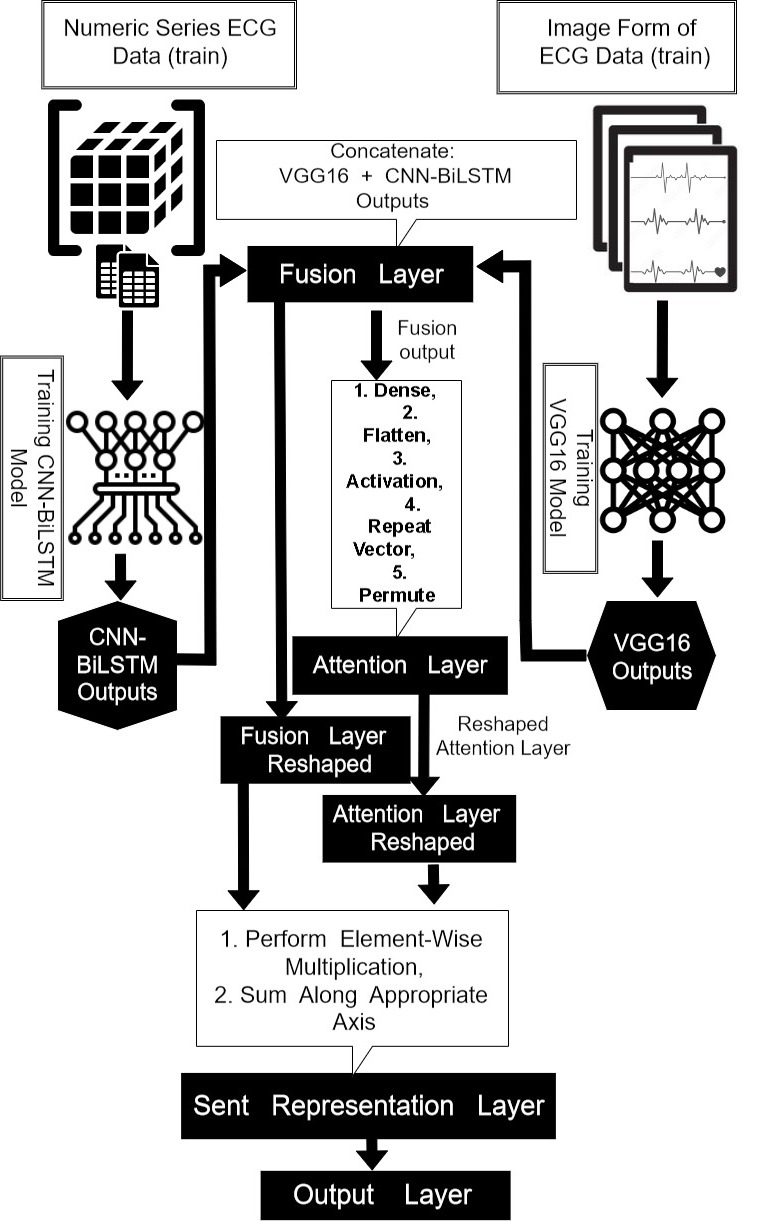
\includegraphics[width=3.5in]{10-Multi-Model.jpg}}
\caption{Architecture of multimodal approach.}
\label{fig-10:multimodal}
\end{figure}
 
Fig. \ref{fig-10:multimodal} shows the multimodal approach, which will improve the classification accuracy hopefully, using both the image and the numerical series data of the ECG signals. In addition, this approach combines a CNN model based on VGG16 for image data and a CNN-BiLSTM model for numerical data. The integration of these networks allows the model to extract information from both data types, which is complementary to the other.

The VGG16 model is pre-trained with the last fully connected layers removed, which extracts features from ECG images and encodes the spatial information.

\begin{equation}
F_{image} = VGG16(X_{image})    
\end{equation}

where, \( X_{image} \) represents the input image data, and \( F_{image} \) denotes the extracted features.

On the other hand, the CNN-BiLSTM model was proposed to handle numerical ECG data by capturing both the local and long-term features. The CNN component of the model extracts local features in the ECG data using filters that help identify features such as peaks and valleys that are important in the analysis of cardiac signals. The next component is BiLSTM, which captures the sequential nature of the data and the long-term dependencies and temporal relationships that are important in the classification and prediction of cardiac conditions. This dual approach guarantees that the model captures fine details in the data while having a global view of the temporal evolution of the ECG signals.

\begin{equation}
F_{numeric} = CNN-BiLSTM(X_{numeric})   
\end{equation}



where, \( X_{numeric} \) is the input numerical data, and \( F_{numeric} \) represents processed features.

The outputs of these models were stitched together to form a fused feature vector that integrates visual and temporal information. This method comprehensively represents the data, merging the benefits of various models; CNNs capture visual-spatial characteristics, and LSTMs capture sequential temporal trends. The formed feature vector provides a robust input for subsequent analysis, using multidimensional data to improve predictive accuracy.


\begin{equation}
F_{fusion} = F_{image} \oplus F_{numeric}
\end{equation}

where \( \oplus \) denotes the concatenation operation.

Subsequently, this model computes a weighted sum of attention vectors on the concatenated feature representation. Moreover, it assigns larger weights to more significant features, enhancing predictive accuracy by focusing on crucial aspects. The relevance scores of each feature, indicating how well it relates to the task, were computed using a dense layer. These scores were then used to normalize the attention weights, ensuring that the sum of all weights is one, highlighting the features that contribute the most to the prediction rather than the less relevant information.

\begin{equation}
a_i = \tanh(W_a \cdot F_{fusion,i} + b_a)
\end{equation}
\begin{equation}
\alpha_i = \frac{\exp(a_i)}{\sum_j \exp(a_j)}
\end{equation}

Here, \( W_a \) and \( b_a \) are the weights and biases of the dense layer, and \( \tanh \) is the hyperbolic tangent activation function. \( \alpha_i \) represents the attention weight for the \( i \)-th feature.

The attention weights are then used to scale the fused features, creating a weighted feature representation that emphasizes essential features. 

\begin{equation}
r = \sum_i \alpha_i \cdot F_{fusion,i}
\end{equation}

This weighted representation \( r \) is the sum of the original characteristics, each multiplied by its weight. In addition, this weighted sum ensures that more important features are given more weight while less important features are given less weight. Subsequently, we reshape the attention and fusion layers to prepare for element-wise multiplication in the subsequent silent representation layer. This process of reshaping the data helps to prepare it for further enhancement of feature interactions and integration in the next step. Finally, the classification layer uses a sigmoid activation function suitable for binary classification problems in the weighted feature representation. Eventually, this activation function maps the sum of the features to a probability score, aiding in identifying the class label and thus solving the binary classification problem.

\begin{equation}
\hat{y} = \sigma(W_c \cdot r + b_c)
\end{equation}

Here, \( W_c \) and \( b_c \) are the weights and biases of the classification layer, and \( \sigma \) is the sigmoid activation function. The output \( \hat{y} \) is the probability value between 0 and 1.

Thus, by combining features from image and numerical data, selecting the most relevant features, and adding the final classification layer, the multimodal model improves the precision of atrial fibrillation classification. This approach emphasizes the model’s capacity to utilize additional data types, improving predictive accuracy and providing a comprehensive solution for AF identification and analysis of atrial fibrillation.


\subsection{Knowledge Distillation}

Knowledge distillation has been accomplished for our series values of the array dataset, considering edge devices. Additionally, it is a technique in which a smaller student model is trained to mimic the behavior of a larger teacher model. This technique allows for the compression of model knowledge and enables the deployment of more efficient models without substantial loss in performance.

\begin{figure}[htbp]
\centerline{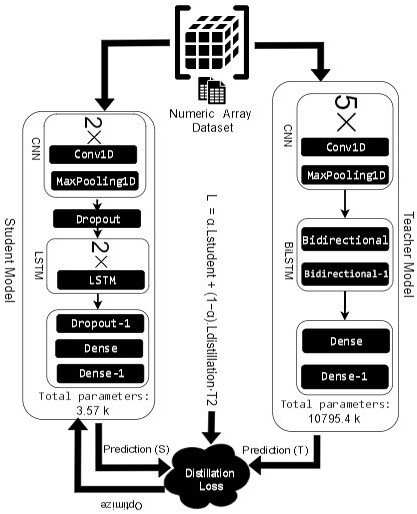
\includegraphics[width=3.5in]{11-KD.jpg}}
\caption{Architecture of multimodal approach.}
\label{fig-11:KD}
\end{figure}

Fig. \ref{fig-11:KD} depicts the knowledge distillation process adopted in this study. In this process, a tiny CNN-LSTM model serves as the student model, while a monster CNN-BiLSTM model acts as the teacher model. In addition, the teacher model, with approximately 10,795.4k parameters, is significantly larger than the student model, which has only 3.57k parameters. Moreover, distillation training combines standard student-loss and distillation-loss, controlled by parameters $\alpha$ and $T$.

The output logits of the teacher model are denoted as $Z_t = \text{teacher}(x)$, and for the student model, they are denoted as $Z_s = \text{student}(x)$ given an input $x$. To soften the logits, the softmax function is applied at temperature $T$:

\begin{equation}
P_t = \text{softmax}\left(\frac{Z_t}{T}\right), \quad P_s = \text{softmax}\left(\frac{Z_s}{T}\right)
\end{equation}

where $P_t$ represents the predictions of the teacher and $P_s$ represents the predictions of the student. The loss of cross-entropy between the true labels $y$ and the predictions of the student model is given by:

\begin{equation}
L_s = \text{Cross-Entropy}(y, \text{softmax}(Z_s))
\end{equation}

The total loss $L$ combines the student loss and the distillation loss, scaled by $\alpha$ and $T^2$:

\begin{equation}
L = \alpha L_s + (1 - \alpha) L_d \cdot T^2
\end{equation}

Here, $L_d$ denotes the distillation loss.

Thus, the student model integrates both student loss and distillation loss, allowing it to mimic the teacher’s predictions effectively while being smaller and more efficient, thus improving its overall performance.

\subsection{Model Evaluation Matrix}

In the final step of the study, we conducted a thorough assessment of the trained models to determine the best-performing model. This evaluation was done using the test dataset and the metrics used included accuracy, F1 score, precision, recall, confusion matrix, AUC score, and ROC curve.


\section{Results and Discussion}


\subsection{ECG Data Acquisition and Analysis} 

In this section, we describe the ECG data acquisition process, signal noise removal, and analysis, as well as the assessment of the AFib detection algorithms used in the developed embedded system. Typical ECG signals mainly consist of several types of waves, one complex, intervals, and segments, as seen in Fig. \ref{fig-12:Typical-ECG-Waveform}.

\begin{figure}[htbp]
\centerline{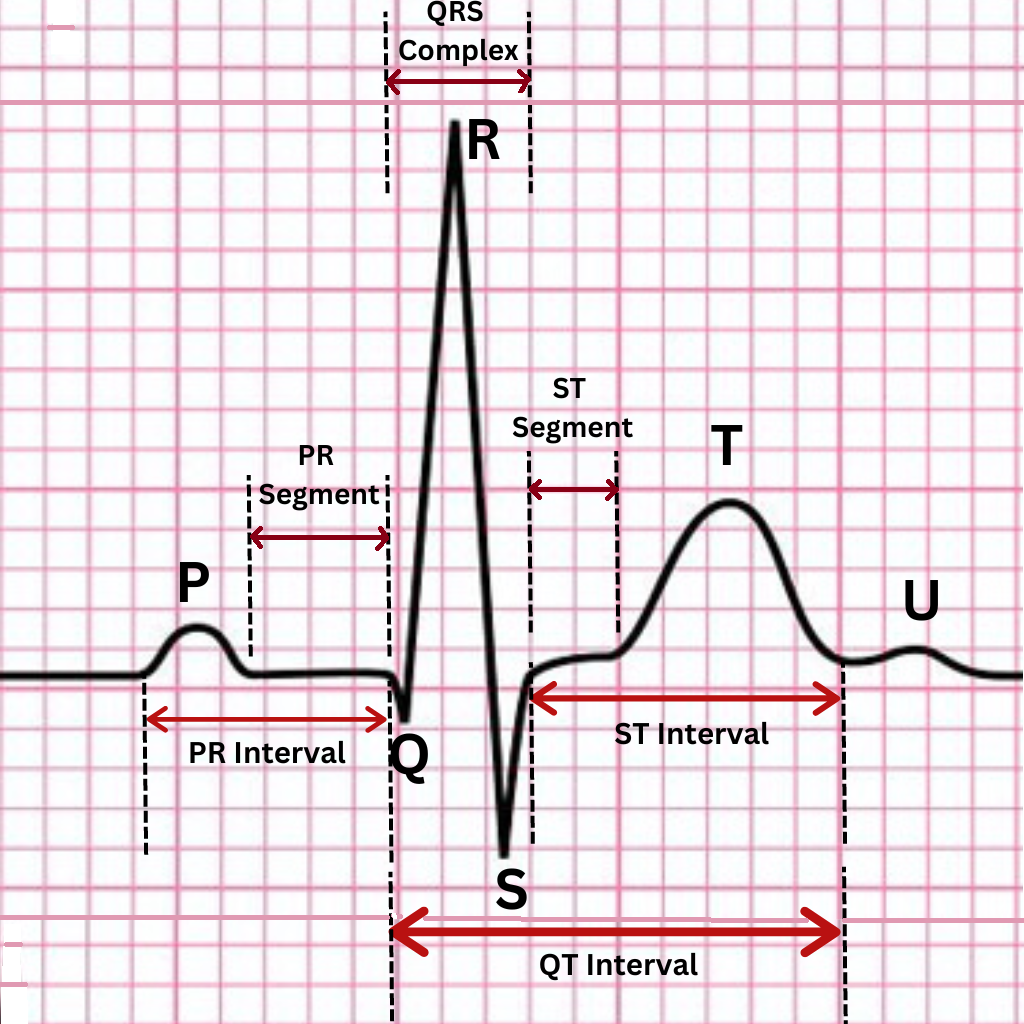
\includegraphics[width=3.5in]{12-Typical ECG webform.png}}
\caption{A Typical ECG Waveform.}
\label{fig-12:Typical-ECG-Waveform}
\end{figure}

\begin{itemize}
    \item \textbf{P Wave:} Represents atrial depolarization.
    \item \textbf{Q Wave:} A slight downward deflection after the P wave.
    \item \textbf{R Wave:} A large upward deflection following the Q wave.
    \item \textbf{S Wave:} A slight downward deflection following the R wave.
    \item \textbf{T Wave:} Represents ventricular repolarization.
    \item \textbf{U Wave:} Sometimes present but usually not seen due to its low peak value.
\end{itemize}

The intervals of these waves are used to diagnose several heart diseases \cite{shaown2019iot}.\\

\textbf{Interval:} Represents the time between two specific ECG waves. The intervals commonly measured on an ECG are the PR interval, QT interval, and RR interval.

\textbf{Segment:} Represents the length between two specific points on an ECG signal that is supposed to be at the baseline amplitude. The segments on an ECG signal include the PR segment and the ST segment.

\textbf{Complex:} The only complex on an ECG signal is the QRS complex.

\begin{figure}[htbp]
\centerline{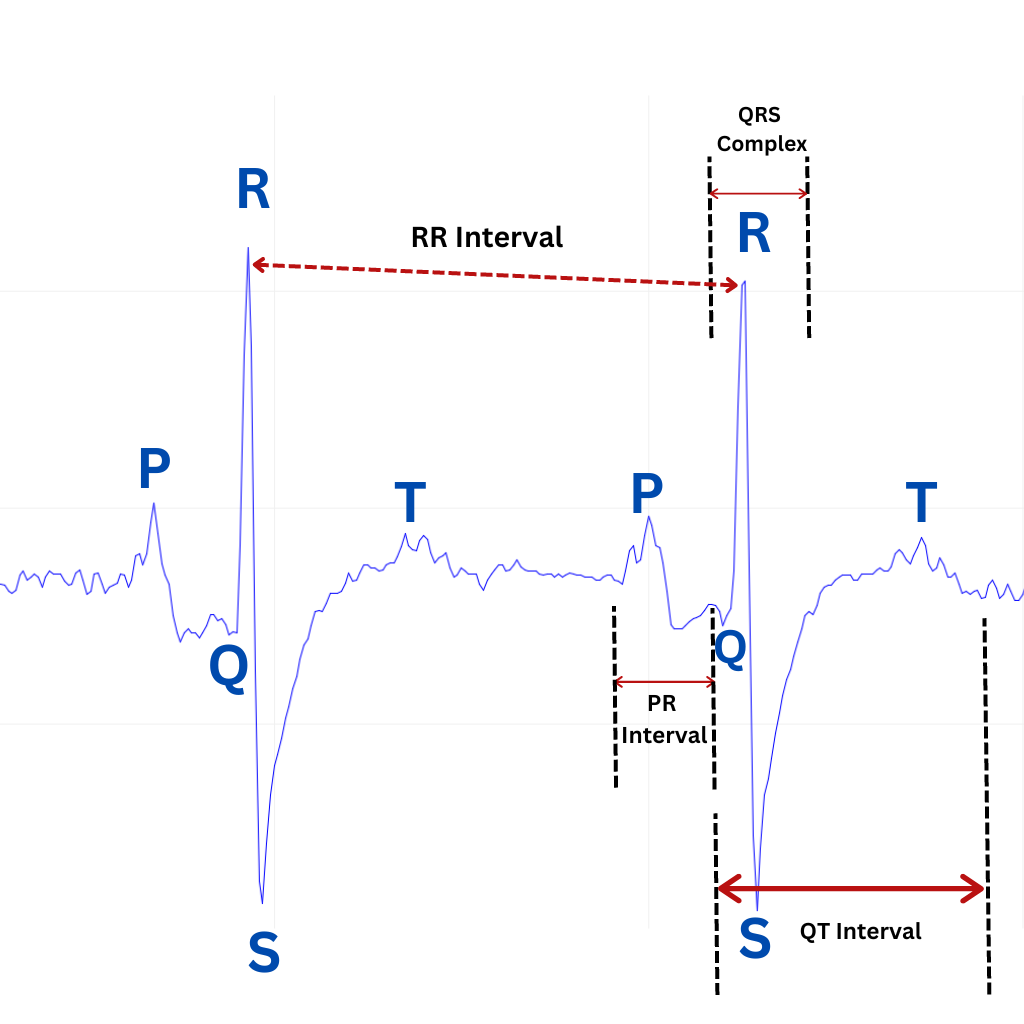
\includegraphics[width=3.5in]{13-Real-time ECG Waveform AD8232.png}}
\caption{Real-time ECG Waveform from AD8232 sensor.}
\label{fig-13:Real-Time-ECG}
\end{figure}

We used the AD8232 single-lead ECG sensor that extracts, amplifies, and filters small bioelectric signals from the human heart. When the three electrodes are typically placed on the right arm (RA), left arm (LA), and right leg (RL), we get a single-lead ECG waveform. The ECG waveform we got from our experiment contains several key components (PR Interval, QRS Complex, and QT Interval) that represent different electrical activities of the heart, as seen in Fig. \ref{fig-13:Real-Time-ECG}.

\textbf{RR Interval:} Indicates the time interval between two adjacent R waves. In arrhythmias, these intervals may become irregular.

\textbf{PR interval:} This measures the time between the beginnings of the P wave and the QRS complex.

\textbf{QRS complex:} Represents Ventricular depolarization, which consists of three essential waves, i.e., Q wave, R wave, and S wave. By analyzing the QRS complex, certain diseases, such as drug toxicity and electrolyte imbalance, are likely to be detected.

\textbf{QT interval:} This represents the time between the beginning of the Q wave and the end of the T wave, which is related to ventricular depolarization and repolarization \cite{shaown2019iot}. If the QT interval exceeds the normal value, there is an increased risk of ventricular fibrillation.

We collected the raw ECG signal values from the Arduino IDE serial monitor for 20.21 seconds at a sampling rate of 99 Hz with a total of 2001 raw ADC values.

\begin{figure}[htbp]
\centerline{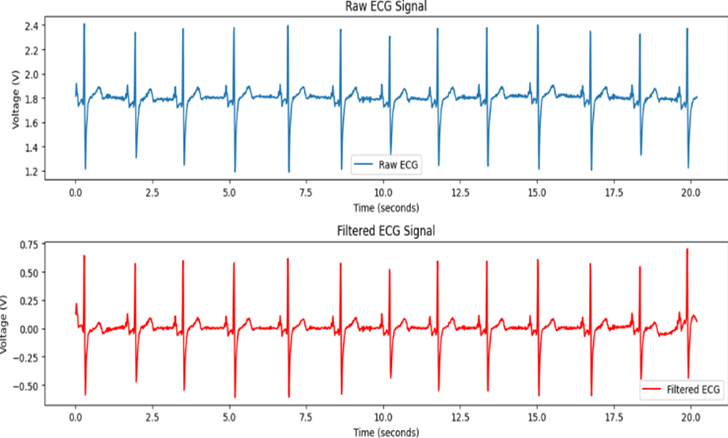
\includegraphics[width=3.5in]{14-Raw Vs. Filtered ECG.png}}
\caption{Raw vs. filtered ECG signal visualization over 20 seconds.}
\label{fig-14:Raw-Vs-Filtered-ECG}
\end{figure}

Fig. \ref{fig-14:Raw-Vs-Filtered-ECG} shows raw and filtered ECG signals where the horizontal axis represents time and the vertical axis represents voltage. The upper panel of the figure depicts the raw ECG signal recorded over approximately 20.21 seconds, showing different peaks of QRS complex, noise, and baseline wandering. The lower panel shows the filtered ECG signal obtained using the band-pass filter that removes high-frequency noise and low-frequency baseline drifts. This process leads to a cleaner signal that preserves the essential characteristics of the ECG waveform, such as P-waves, QRS complexes, and T-waves. The previously created time vector could transform the sample numbers into the actual time in seconds. 

The Raspberry Pi 4 B receives the ECG data from the ESP8266 in a serial fashion and processes the signals to allow the execution of the preloaded deep-learning model for AFib diagnosis. This model was created using Python and incorporated the Keras library with TensorFlow as the backend \cite{ahsanuzzaman2020low}, analyzing the data and offering diagnostic outcomes. Raspberry Pi displays the results at the end of the testing phase.

\subsection{Limitations of Hardware Section}

The AD8232 provides a single-lead ECG, which is helpful for essential heart rate monitoring and detecting some arrhythmias. Still, it does not offer the comprehensive diagnostic capabilities of a multi-lead or 12-lead ECG system because it may lack the fine detail and spatial resolution of a 12-lead ECG.

We get a single view of the heart’s electrical activity. Moreover, the proposed system is useful for monitoring heart rate and detecting significant arrhythmias such as Atrial Fibrillation. However, it is limited in its ability to diagnose more complex cardiac conditions. Therefore, the quality and accuracy of the waveform depend on proper electrode placement and good contact with the skin.


\subsection{Model Evaluation on ECG Dataset}

To obtain a more realistic assessment of the proposed system, we need to apply several evaluation criteria. These were the accuracy matrix, F1-score, precision, recall, confusion matrix, AUC-ROC, and ROC curve. This assessment strategy is effective for providing a broad evaluation of the diagnostic functions of the system and its effectiveness in identifying atrial fibrillation.

The three trained models were thoroughly assessed in the form of the ECG dataset in the test data, which was 20\% of the entire dataset. Table I presents the accuracy, precision, recall, and F1 score of these models after 80 epochs of training, which gives a quantitative measure of the efficiency of the proposed models.

\begin{table}[!ht]
\centering
\caption{Performance metrics for array form of ECG data.}
\label{tab:array_ecg}
\begin{tabularx}{\columnwidth}{|X|X|X|X|X|}
\hline
Model & Accuracy (\%) & Precision & Recall & F1-Score \\
\hline
LSTM & 71.24 & 0.71 & 0.71 & 0.71 \\
\hline
CNN-LSTM & 89.41 & 0.89 & 0.89 & 0.89 \\
\hline
CNN-BiLSTM & 92.73 & 0.93 & 0.92 & 0.93 \\
\hline
\end{tabularx}
\end{table}

In Table \ref{tab:array_ecg}, it is evident that the CNN-BiLSTM model outperforms the others, making it the most effective model for the array form of the ECG dataset.

We also evaluated three trained models using the image form of the ECG dataset on the test data, also comprising 20\% of the total dataset. Table II presents the performance metrics—accuracy, precision, recall, and F1-score—of these models.

\begin{table}[!ht]
\centering
\caption{Performance Metrics of Different Models.}
\begin{tabularx}{\columnwidth}{|X|X|X|X|X|X|}
\hline
Model & Accuracy (\%) & Precision & Recall & F-1 & Params (k) \\ \hline
ViT & 83.57 & 0.83 & 0.83 & 0.82 & 63200 \\ \hline
ResNet32 & 85.65 & 0.86 & 0.86 & 0.86 & 49278.6 \\ \hline
VGG16 & 89.97 & 0.90 & 0.90 & 0.90 & 165.5 \\ \hline
\end{tabularx}
\label{tab:performance_metrics}
\end{table}

From the analysis in Table \ref{tab:performance_metrics}, we can determine that VGG-16 our best performing model on image dataset.

\subsection{Performance of Multimodal Approach}

Since we identified the CNN-BiLSTM and the VGG16 models as the best-performing models for each data form from Table 2 and Table 3, we integrated them into the proposed multimodal approach to improve the performance. Table III shows the type of data, training accuracy, validation accuracy, and validation loss of the individual and multimodal models.

\begin{table}[!ht]
\centering
\caption{Comparison between Unimodal and Multimodal Models.}
\begin{tabularx}{\columnwidth}{|X|X|X|X|X|}
\hline
\textbf{Type of Data} & \textbf{Model} & \textbf{Train Accuracy} &  \textbf{Validation Accuracy} & \textbf{Validation loss} \\
\hline
Image & VGG16 (Unimodal) & 92.31 & 89.89 & 0.45 \\
\hline
Digital & CNN-BiLSTM (Unimodal) & 97.43 & 92.73 & 0.36\\
\hline
Digital-Image & VGG16 + CNN-BiLSTM (Multimodal) & 98.35 &  94.01 & 0.24 \\
\hline
\end{tabularx}
\label{table:multimodal}
\end{table}
 
From Table \ref{table:multimodal}, we can conclude that the multimodal approach, which integrates the best models from both data forms, achieves a superior performance compared to individual models.

\subsection{Performance of Knowledge Distillation}

To assess the performance of KD, we compared the CNN-LSTM model with the CNN-BiLSTM model and the CNN-LSTM model after applying KD. Table \ref{table:knowledge_distillation} shows the accuracy, precision, recall and F1 score of the proposed model.

\begin{table}[!ht]
\centering
\caption{Performance metrics for knowledge distillation.}
\begin{tabularx}{\columnwidth}{|X|X|X|X|X|}
\hline
Model & Accuracy (\%) & Precision & Recall & F1-Score \\
\hline
CNN-LSTM (Student) & 75.41 & 0.75 & 0.75 & 0.75 \\
\hline
CNN-BiLSTM (Student) & 93.73 & 0.93 & 0.93 & 0.93 \\
\hline
Student After KD & 83.01 & 0.83 & 0.82 & 0.82 \\
\hline
\end{tabularx}
\label{table:knowledge_distillation}
\end{table}

According to Table \ref{table:knowledge_distillation}, it is evident that knowledge distillation significantly improves the performance of the student model, making it a viable option for deployment on edge devices with limited computational resources.

Therefore, the evaluation of the proposed approach proved that the CNN-BiLSTM model was the best for the array form of the ECG dataset, while the VGG16 model was the best for the image form of the dataset. The results of the multimodal approach, which combines the features of both models, were the highest. Moreover, knowledge distillation is useful for fine-tuning models for edge devices, which proves its effectiveness in real-world scenarios.


\subsection{Sample Input in Knowledge Distillation Model from Hardware Output}

We collected the sample using hardware, and put the sample into the KD student model as an input after preprocessing. We collected the hardware sample as a CSV file, and we prepared that file for the trained model input. In detail, we converted the CSV into a 3D array of series values. Then, we passed the input to the preprocessing pipeline to prepare it as an input for our KD model. Eventually, the model was prepared to predict Normal SR or Atrial fibrillation. 

\subsection{Model Evaluation Using Confusion Matrix}

When a table displays the counts of true positives, true negatives, false positives, and false negatives for a classification model, it is a confusion matrix. In addition, it provides detailed insight into whether the predictions of the model were correct or incorrect. Eventually, this insight allows for the calculation of performance metrics like accuracy, precision, recall, and F1-score, which are crucial for assessing the effectiveness of the model.

\begin{figure}[htbp]
\centerline{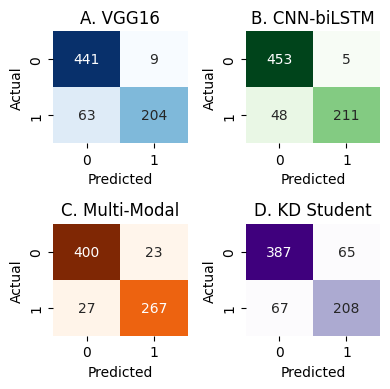
\includegraphics[width=3.5in]{15-Confusion Matrix.png}}
\caption{Confusion matrices for the considered models: (A) VGG16, (B) CNN-BiLSTM, (C) Multi-Modal (D) KD Student.}
\label{fig-15:CM}
\end{figure}

In the confusion matrix in Fig. \ref{fig-15:CM}, we can observe that for the ECG image form of data, the  VGG16 model could predict the 'Normal' samples very well, but it was not that accurate in predicting the other class. On the other hand, we observe the same case with CNN-BiLSTM for the array version of the same data. That means both models show slightly biased behavior for the 'Normal' class. Then, if we study the confusion matrix (c), we will realize that the multi-modal approach successfully reduced the biasedness of the class 'Normal' and dealt with both classes of data from the fairground. Therefore, we can observe improvement in the quality of learning by applying the multi-modal model. Moreover, in the confusion matrix (d), the knowledge distillation student model shows fair behavior like the multi-modal model, though its prediction accuracy wasn't premier like the multi-modal model.


\subsection{Model's Activity Interpretation Using XAI}

To gain more insight into the focus of the model and the decision-making process, we employ an able-bodied AI method known as Local Interpretable Model-Agnostic Explanations (LIME). LIME enables the interpretation of individual predictions by determining whether our VGG16 model focuses on the relevant areas of the ECG images. It does so by assuming the model to be a black box and only needing to have access to the model’s predictions while creating easily interpretable visualizations such as heatmaps.

\begin{figure}[htbp]
\centerline{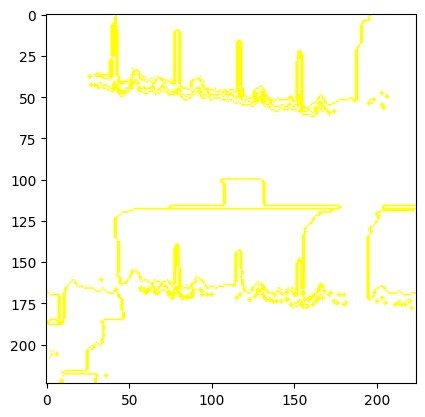
\includegraphics[width=3.5in]{16-LIME.jpg}}
\caption{A heatmap, produced by LIME.}
\label{fig-16:LIME}
\end{figure}

Fig. \ref{fig-16:LIME} shows that a heatmap has been produced by LIME to interpret the inner activity of the VGG16 model with the ECG images during model training. From the heatmap, we can conclude that the VGG16 model was properly paying attention to the right areas. Therefore, everything was going on superbly inside the model when the training was going on.
Evaluating machine learning and deep neural network models’ performance goes beyond a single view. We measured the models’ accuracy and optimistic predictive ability using measures such as accuracy and precision. Analyzing metrics, like accuracy, precision, recall, and the confusion matrix, helped us understand how well the model identified true positives, classified overall, and predicted unseen data, ultimately leading to better model improvement and selection for specific tasks.

This evaluation allowed us to determine which performance metrics are the most accurate and reliable for the heart disease diagnosis system. The approach of evaluating all the models and then using LIME for interpretability helped us select a model that was not only just accurate but also explainable.

In conclusion, strict evaluation and the application of explainable AI methods allow us to understand the performance and interpretability of the model in detail. This approach helped to choose the most suitable model for the correct and efficient diagnosis of heart diseases, which improved the performance of the diagnostic system.

\subsection{Comparing Our Work with Existing Systems}

Comparing existing systems with our system is a very intuitive discussion, but it is necessary to point attention to the newly discovered improvements in this specific field. In other words, answering the question of why this study is meaningful and worthy.

\begin{table}[!ht]
\centering
\caption{Comparison table of our system vs existing systems.}
\begin{tabularx}{\columnwidth}{|c|X|c|X|}
\hline
No & Our System & vs & Existing Systems \\ \hline
1 & Our study used only 3 ECG leads to detect Atrial Fibrillation. & & No other study did better than us using the PTB-XL dataset.\\ 
\hline
2 & We generate the ECG image dataset from PTB-XL raw signals for the multi-modal approach. & & No other study did a similar thing. \\ 
\hline
3 & We explored the multi-modal approach for the PTB-XL dataset. & & No other study did that.\\ 
\hline
4 & Our system has real-time ECG-taking capability for detection. & & Some study has that but not cost-effective like us. \\ 
\hline
5 & Our study explored the multimodal approach, KD for edge devices, and an embedded system for Afib detection from ECG. & & No other study explored all those things together.\\ 
\hline
6 & Our multimodal accuracy value 94, is promisingly good, but not the best. Moreover, our KD accuracy was 83, which could have been far better. & & Many existing studies had better accuracy than us.  \\ 
\hline
\end{tabularx}
\label{tab:comparison vs other study}
\end{table}

Therefore, from Table \ref{tab:comparison vs other study}, we can conclude that this study explored a vast range, and at the same time it is better than many other recent existing systems.

\subsection{Limitations of The Machine Learning Part}

\begin{itemize}
    \item \textbf{1.} Our system can detect whether it is an Atrial fibrillation or a normal ECG signal. If it could detect other heart diseases from the ECG signals, it would be beautiful.
    \item \textbf{2.} Our multimodal accuracy value 94, is promissingly good, but not the best. If it was more than 98\%, then, it would be perfect.
    \item \textbf{3.} Moreover, our KD accuracy was 83, which is average for recent times. It could have been far better.
    \item \textbf{4.} It could have been a low-cost tiny device, where our AI system was integrated.
\end{itemize}


\section{Conclusion}

In this work, we present a new system that includes sensors, microcontrollers, and complex signal processing for real-time ECG monitoring. Bluetooth is applied to connect the AD8232 sensor, ESP8266, and Raspberry Pi 4B; the battery power source is an essential aspect of mobility that transforms our solution into a handy tool for monitoring one's health in mobile mode. Thus, by fine-tuning machine learning deep learning models and hyperparameters, we have broadened the range of cardiac analysis and examined other characteristics that make the system robust. The data preprocessing and training of the models exhibited worthwhile outcomes. These results confirm the precision of the proposed method for the classification and prediction of cardiac conditions with high accuracy.

Our future development plan for the system is to have a web application that will enhance connectivity and accessibility to users to make it easy to use and be the central point for real-time ECG monitoring for the entire system. This application will serve as a centralized platform for real-time ECG monitoring, providing an intuitive interface for users to track their heart activity and access real-time ECG data. Through the integrated WIFI of the ESP8266, the sensors, and the mobile application, users may examine their ECG results in real time. This user-centered approach ensures that health problems are detected early and cardiac assessment is made easily understandable to the public.

In this case, we present a general approach that can be applied to solve problems associated with ECG supervision and timely cardiac care. By providing real-time data and analysis to users, our solution is not limited to ECG monitoring, which improves our mission of patient-centered preventive healthcare. Further, the system also provides an understanding of future advancements in health monitoring, which would be the scope for further advancement in the healthcare field.

\bibliographystyle{ieeetr}
\bibliography{1-A-Refrence.bib}


% % Your document content...

% % References section
% \begin{thebibliography}{99}

%\end{thebibliography}
\end{document}

















 

























 
